\documentclass[letterpaper,11pt]{article}

%%%%%%%%%%%%%%%%%%%%%%%%%%%%%%%%%%%%%%%%%%%
%	PAQUETES
%%%%%%%%%%%%%%%%%%%%%%%%%%%%%%%%%%%%%%%%%%%

\usepackage[spanish]{babel}
\usepackage[left=2.5cm,right=2.5cm,top=2.5cm,bottom=2.5cm]{geometry}
\usepackage{graphicx}
\usepackage{float}
\usepackage{subcaption}

%%%%%%%%%%%%%%%%%%%%%%%%%%%%%%%%%%%%%%%%%%%%%%%
%	PORTADA
%%%%%%%%%%%%%%%%%%%%%%%%%%%%%%%%%%%%%%%%%%%%%%%

\begin{document}
	\begin{titlepage}
		%------------------------------------------------
		% ENCABEZADO
		%------------------------------------------------
		\noindent
		\begin{minipage}[t]{0.60\textwidth}
			\begin{minipage}[t]{0.22\textwidth}
				\vspace{0pt}
				
\includegraphics[width=1.8cm]{Img/logo_UdeC.png}
			\end{minipage}
			\hfill
			\begin{minipage}[t]{0.72\textwidth}
				\vspace{0pt}
				\small
				Departamento de Ingeniería Eléctrica\\
				Facultad de Ingeniería\\
				Universidad de Concepción
			\end{minipage}
		\end{minipage}
		\hfill
		\begin{minipage}[t]{0.35\textwidth}
			\vspace{0pt}
			\raggedleft
			
\includegraphics[width=\linewidth]{Img/logo_ICT.png}
		\end{minipage}
		%------------------------------------------------
		% TÍTULO
		%------------------------------------------------
		\vfill
		\begin{center}
			{\Huge\bfseries 549305 -- TIC 2}
			\vspace{0.6cm} \\
			{\LARGE\bfseries Proyecto Final}
		\end{center}
		\vfill
		%------------------------------------------------
		% INFORMACIÓN
		%------------------------------------------------
		\begin{center}
			\begin{tabular}{rl}
				\textbf{Profesor:} & Vincenzo Caro Fuentes
				\\[0.4cm]
				\textbf{Integrantes:} & Matthias Aliaga Febres
				\\ & Alan Haro Cárdenas
			\end{tabular}
			\vspace{1.2cm} \\
			\today, Concepción, Chile
		\end{center}
	\end{titlepage}

%%%%%%%%%%%%%%%%%%%%%%%%%%%%%%%%%%%%%%%%%%%%%%%%%%%%
%	PÁGINA 1
%%%%%%%%%%%%%%%%%%%%%%%%%%%%%%%%%%%%%%%%%%%%%%%%%%%%

\newpage
\section{Descripción general del proyecto}
\noindent En esencia la idea del proyecto consiste en una puerta automática con cerradura electrónica que se abre al pasar por un lector una tarjeta o un llavero autorizado. \\

\noindent Podemos dividir el funcionamiento de la parte electrónica del proyecto en dos partes. La electrónica que controla la puerta y la que controla los servomotores que abren la puerta y la hacen automática.


\subsection{CIRCUITO PUERTA}
\begin{figure}[H]
	\centering
	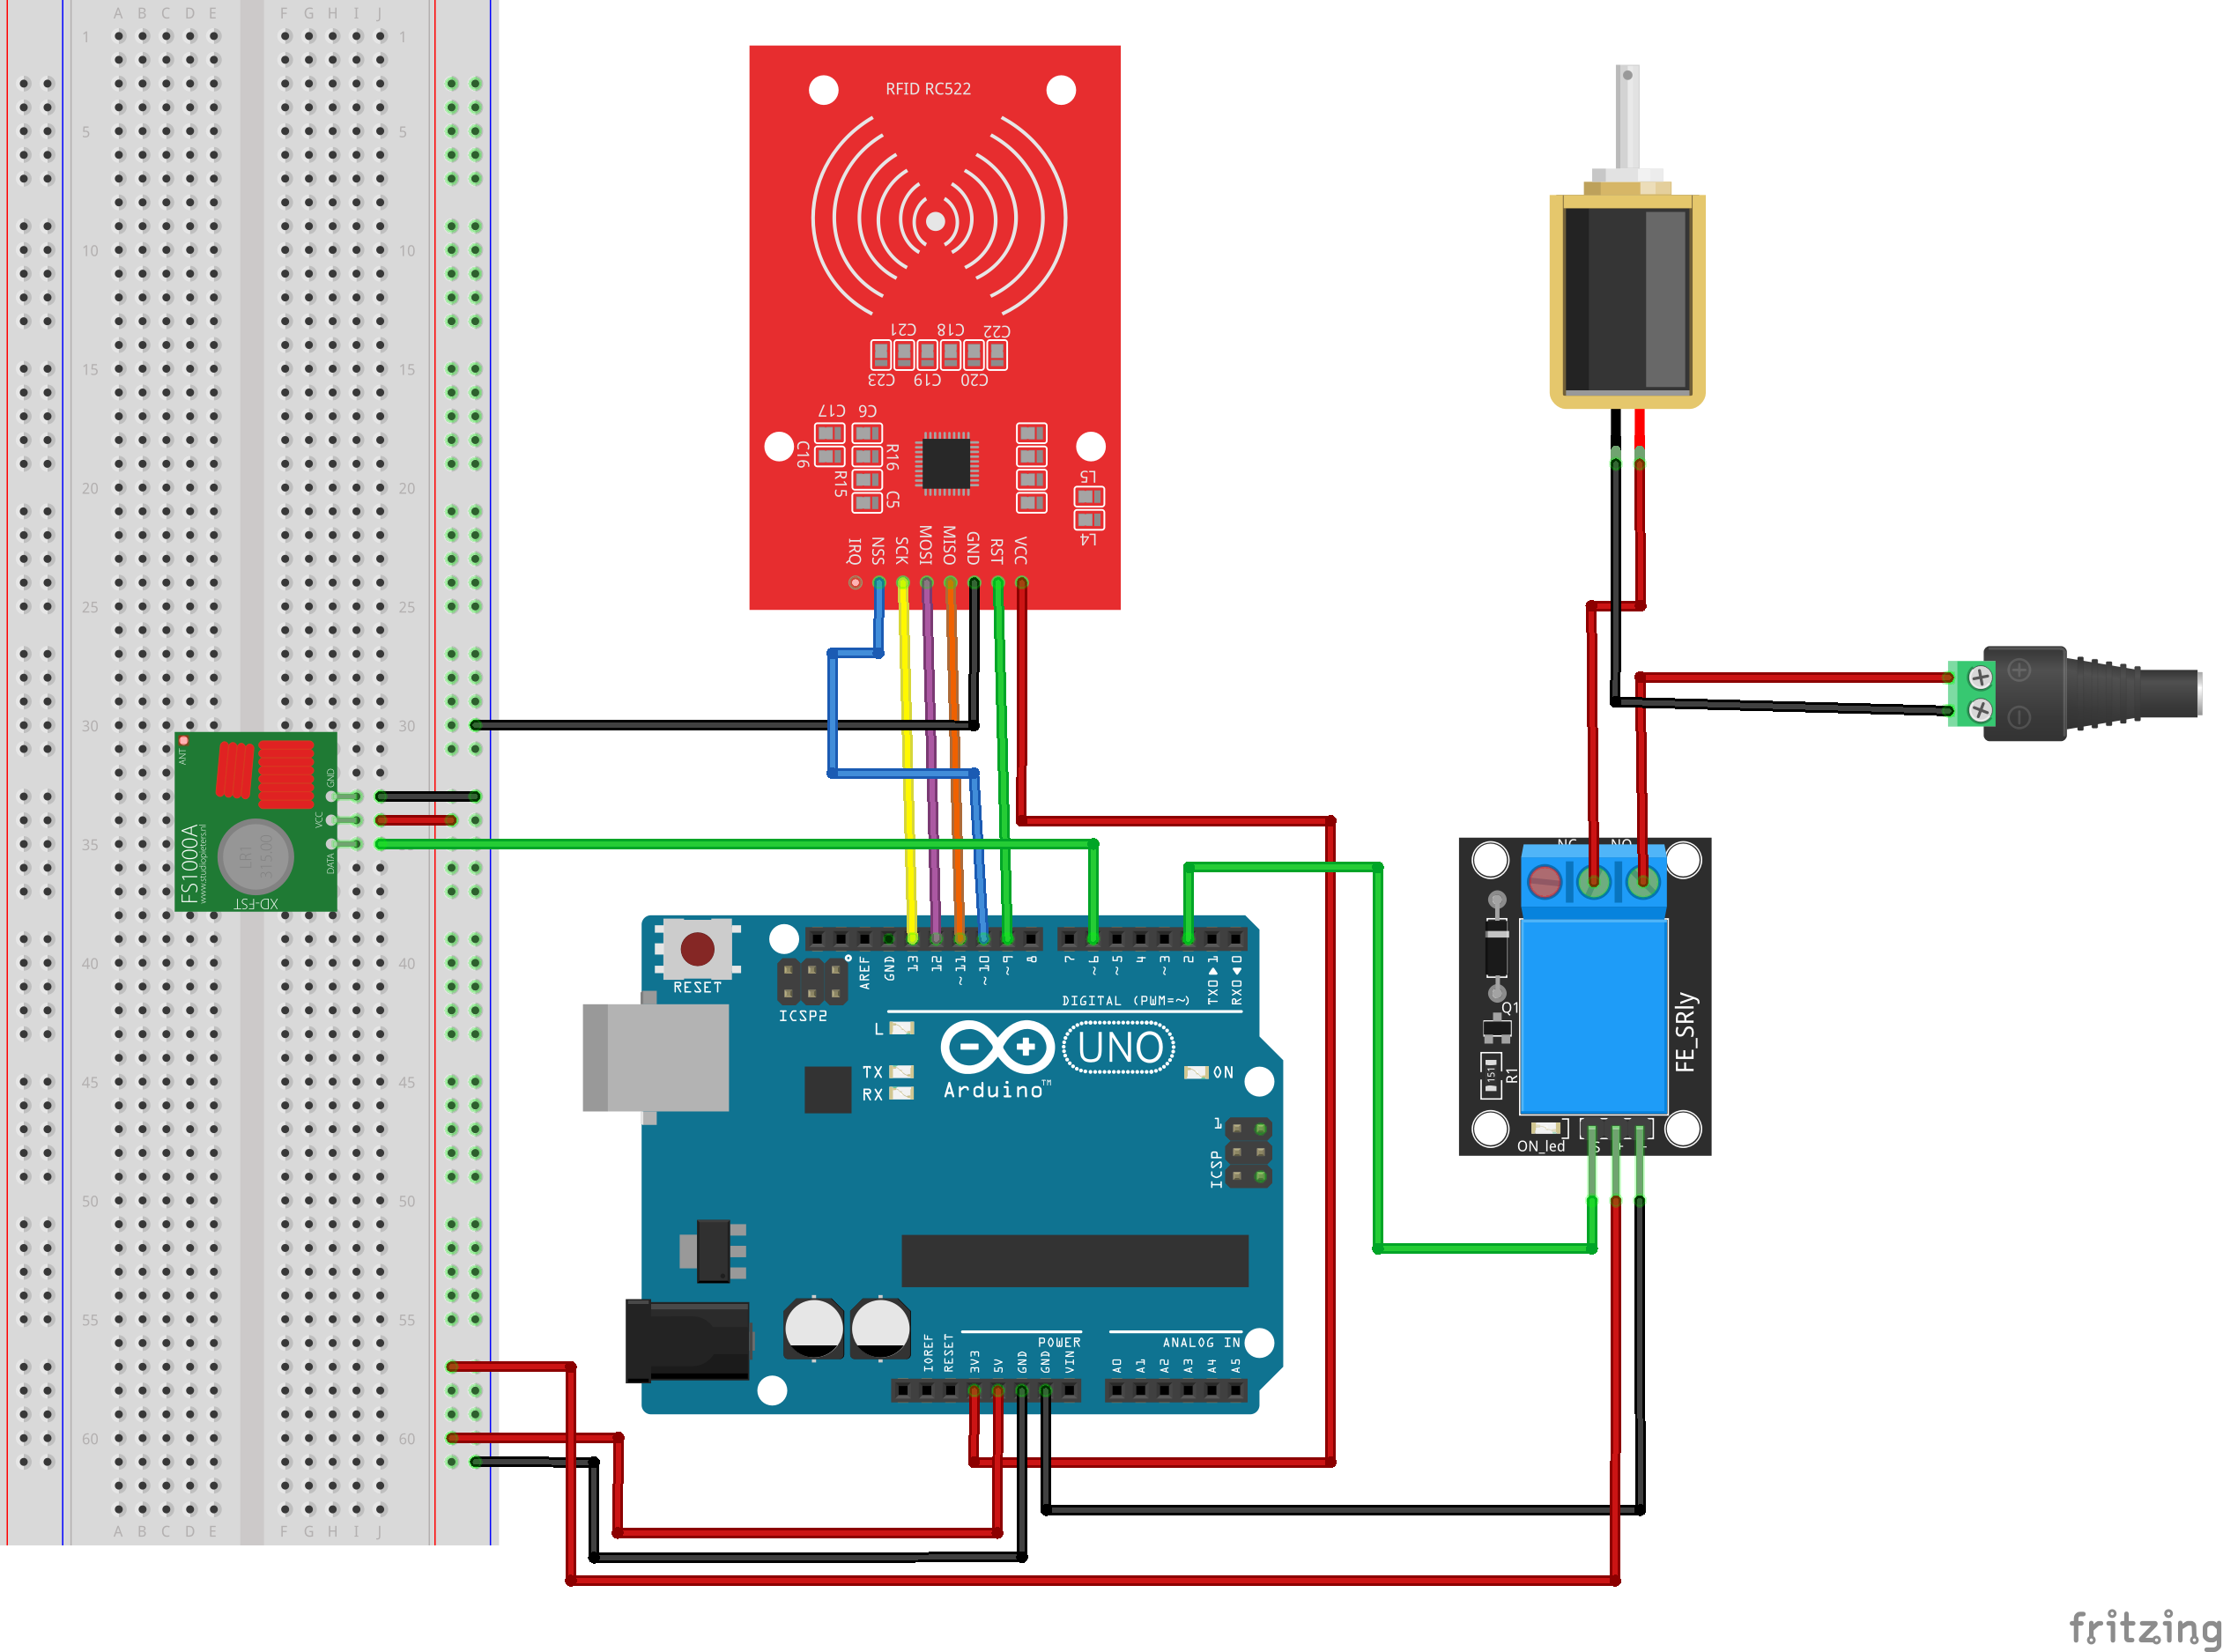
\includegraphics[width=0.6\linewidth]{Img/circuito_puerta_img}
	\caption{circuito puerta}
	\label{fig:circuitopuertaimg}
\end{figure}


\subsubsection{Funcionamiento solenoide - relé - fuente de poder}
\noindent Para el pestillo de la puerta se usó un solenoide de 12v, la energía que consumia este era demasiado para la placa de arduino por tanto se tuvo que usar también una fuente de poder individual (12v 3a) en conjunto con un adaptador hembra. Era necesario además tener una manera de comunicar la placa de arduino con el solenoide pues este solo tiene dos estados: encendido y apagado; para ello se ocupó un relé, este al recibir la instrucción de la placa de arduino dejaba o no pasar corriente hacia el solenoide para encenderlo o apagarlo. 


\subsubsection{Funcionamiento lector RFID - RF emisor 433 mhz}
\noindent Por otra parte para que solo personal autorizado pudiera abrir la puerta se utilizó un lector RFID, este debería estar en todo momento a la espera de una tarjeta o llavero que buscara ser leído. Finalmente como era necesario comunicar el arduino que controla la puerta con el arduino que controla los servomotores se utilizó un módulo RF emisor de 433 mhz. 

%%%%%%%%%%%%%%%%%%%%%%%%%%%%%%%%%%%%%%%%%%%%%%%%%%%%%
%	PÁGINA 2
%%%%%%%%%%%%%%%%%%%%%%%%%%%%%%%%%%%%%%%%%%%%%%%%%%%%%

\newpage
\subsection{CIRCUITO SERVOS}
\begin{figure}[H]
	\centering
	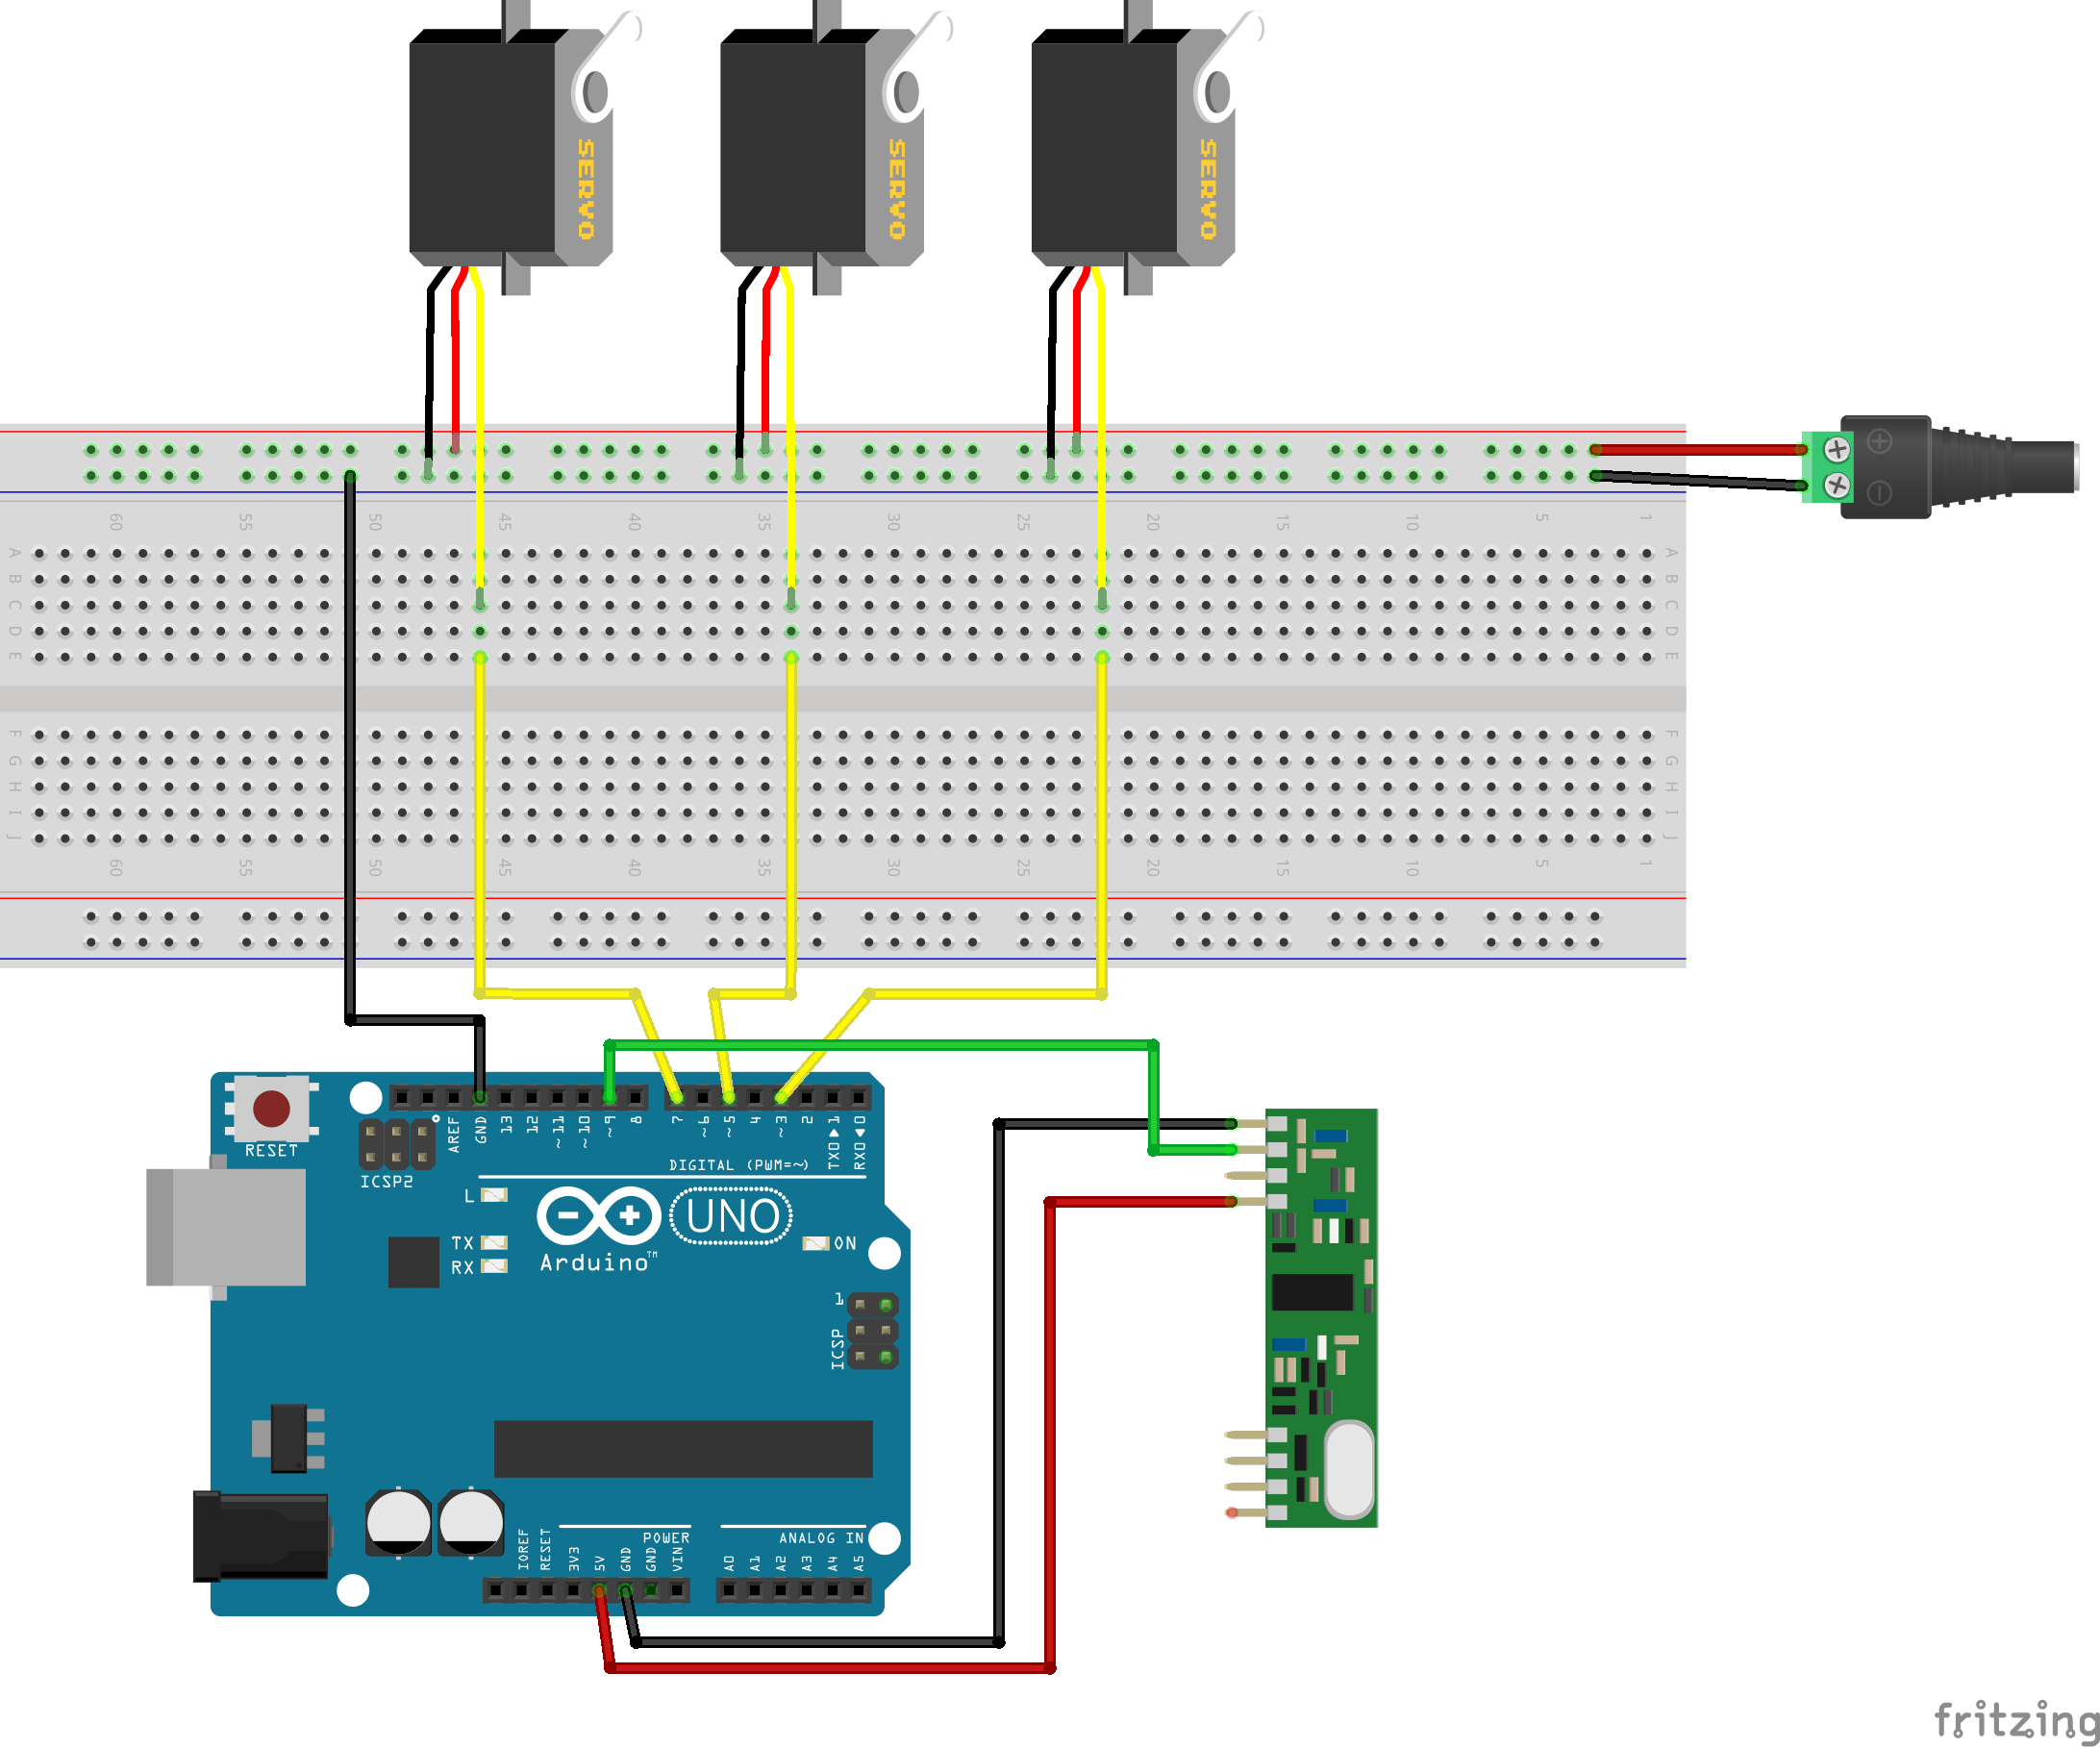
\includegraphics[width=0.6\linewidth]{Img/circuito_servos_img}
	\caption{circuito servos}
	\label{fig:circuitoservosimg}
\end{figure}

\subsubsection{Funcionamiento servos - fuente de poder - RF receptor 433 mhz}
\noindent A máxima capacidad los servos modelo sg90 pueden llegar a consumir hasta 700ma por ello se precisaba de una fuente de poder individual (5v 3a) para poder alimentarlos en conjunto con un adaptador hembra. En el circuito de la sección anterior se enviaba una señal al arduino que controla estos servos a traves de un emisor RF de 433 mhz, para recibir dicha señal se ocupó en este circuito un receptor RF de 433 mhz. \\

\noindent A modo de resumen el siguiente diagrama condensa el funcionamiento completo de la puerta automática:

\begin{enumerate}
	\item La puerta cerrada mantiene activo su lector RFID. 
	\item Una tarjeta o llavero autorizado es escaneado por el lector y este le da la orden a arduino de abrir la puerta.
	\item Arduino envia la señal al relé para que este deje pasar corriente al solenoide y el pestillo se abra.
	\item Con el pestillo abierto el emisor RF envia la señal para mover la puerta al otro arduino controlador de servos la cual es recibida por el receptor RF.
	\item Arduino finalmente le da la orden a los servos para moverse simultáneamente y abrir la puerta. 
\end{enumerate} 

%%%%%%%%%%%%%%%%%%%%%%%%%%%%%%%%%%%%%%%%%%
%	PÁGINA 3
%%%%%%%%%%%%%%%%%%%%%%%%%%%%%%%%%%%%%%%%%%

\newpage
\section{Galería de fotos}
\noindent He aquí algunas fotos del proyecto terminado.

\begin{figure}[H]
	\centering
	\begin{subfigure}{0.45\textwidth}
		\centering
		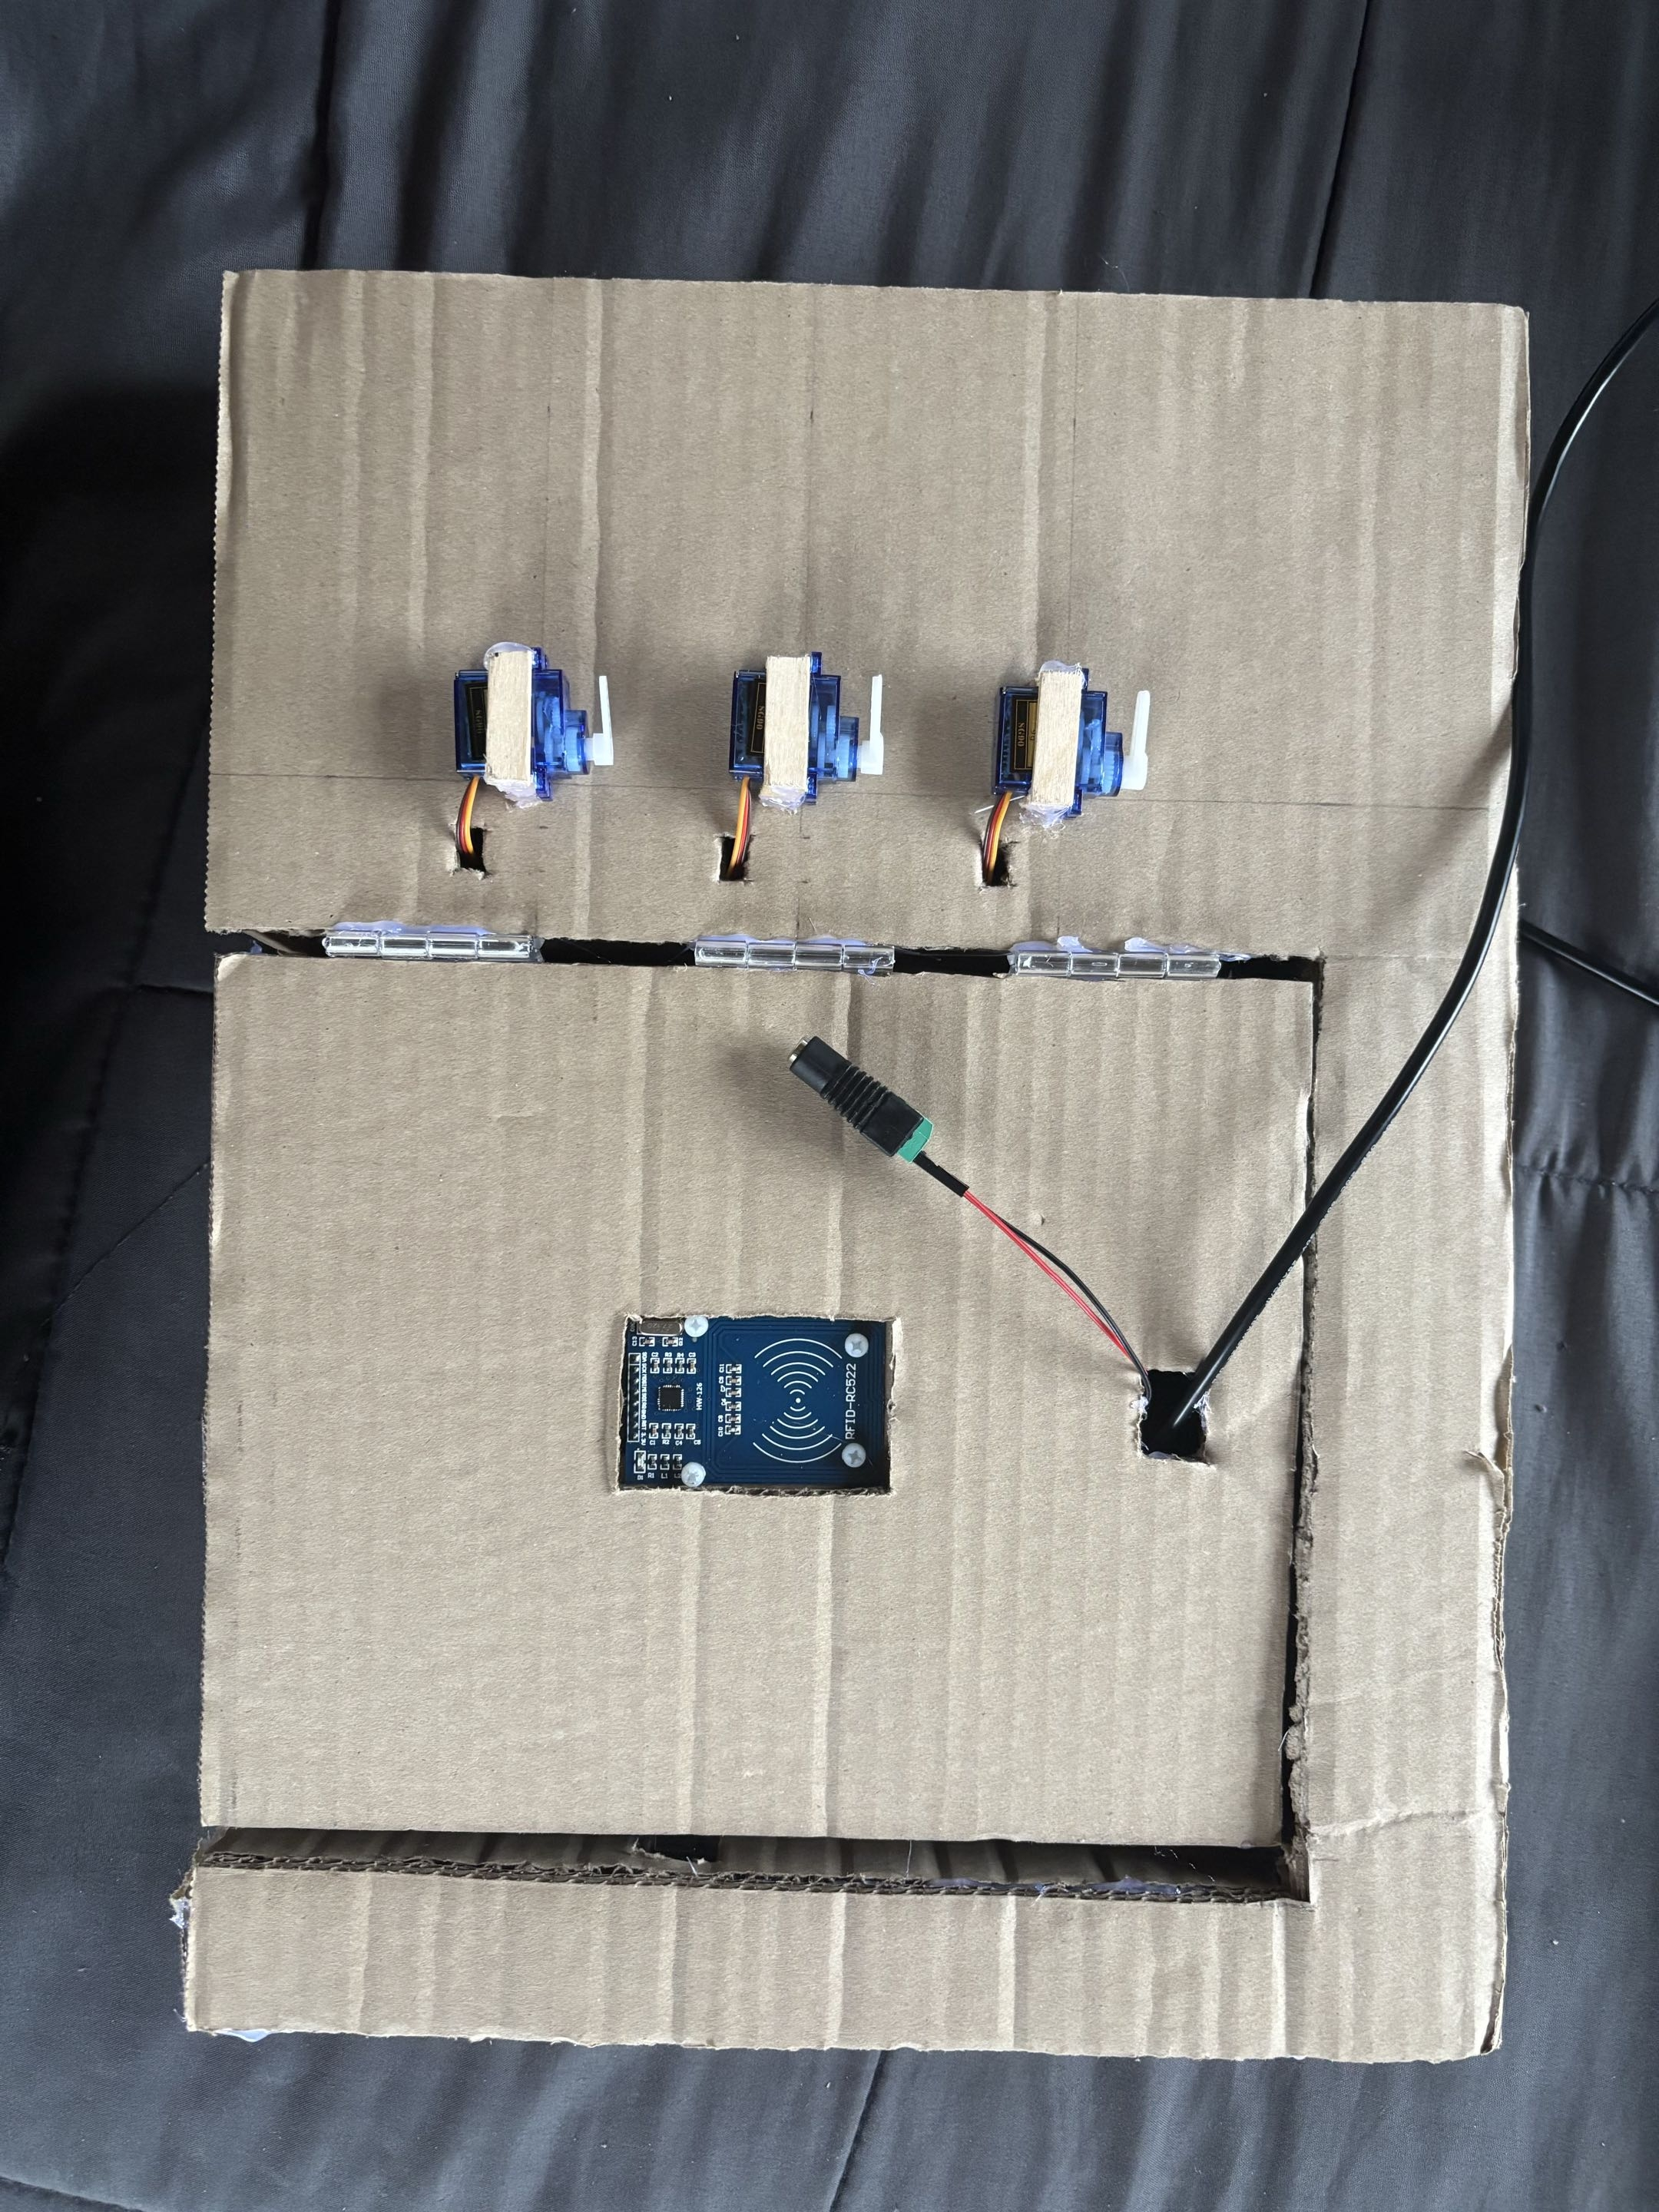
\includegraphics[width=0.6\linewidth]{Img/imagen2}
		\caption{vista frontal}
	\end{subfigure}
	\hfill
	\begin{subfigure}{0.45\textwidth}
		\centering
		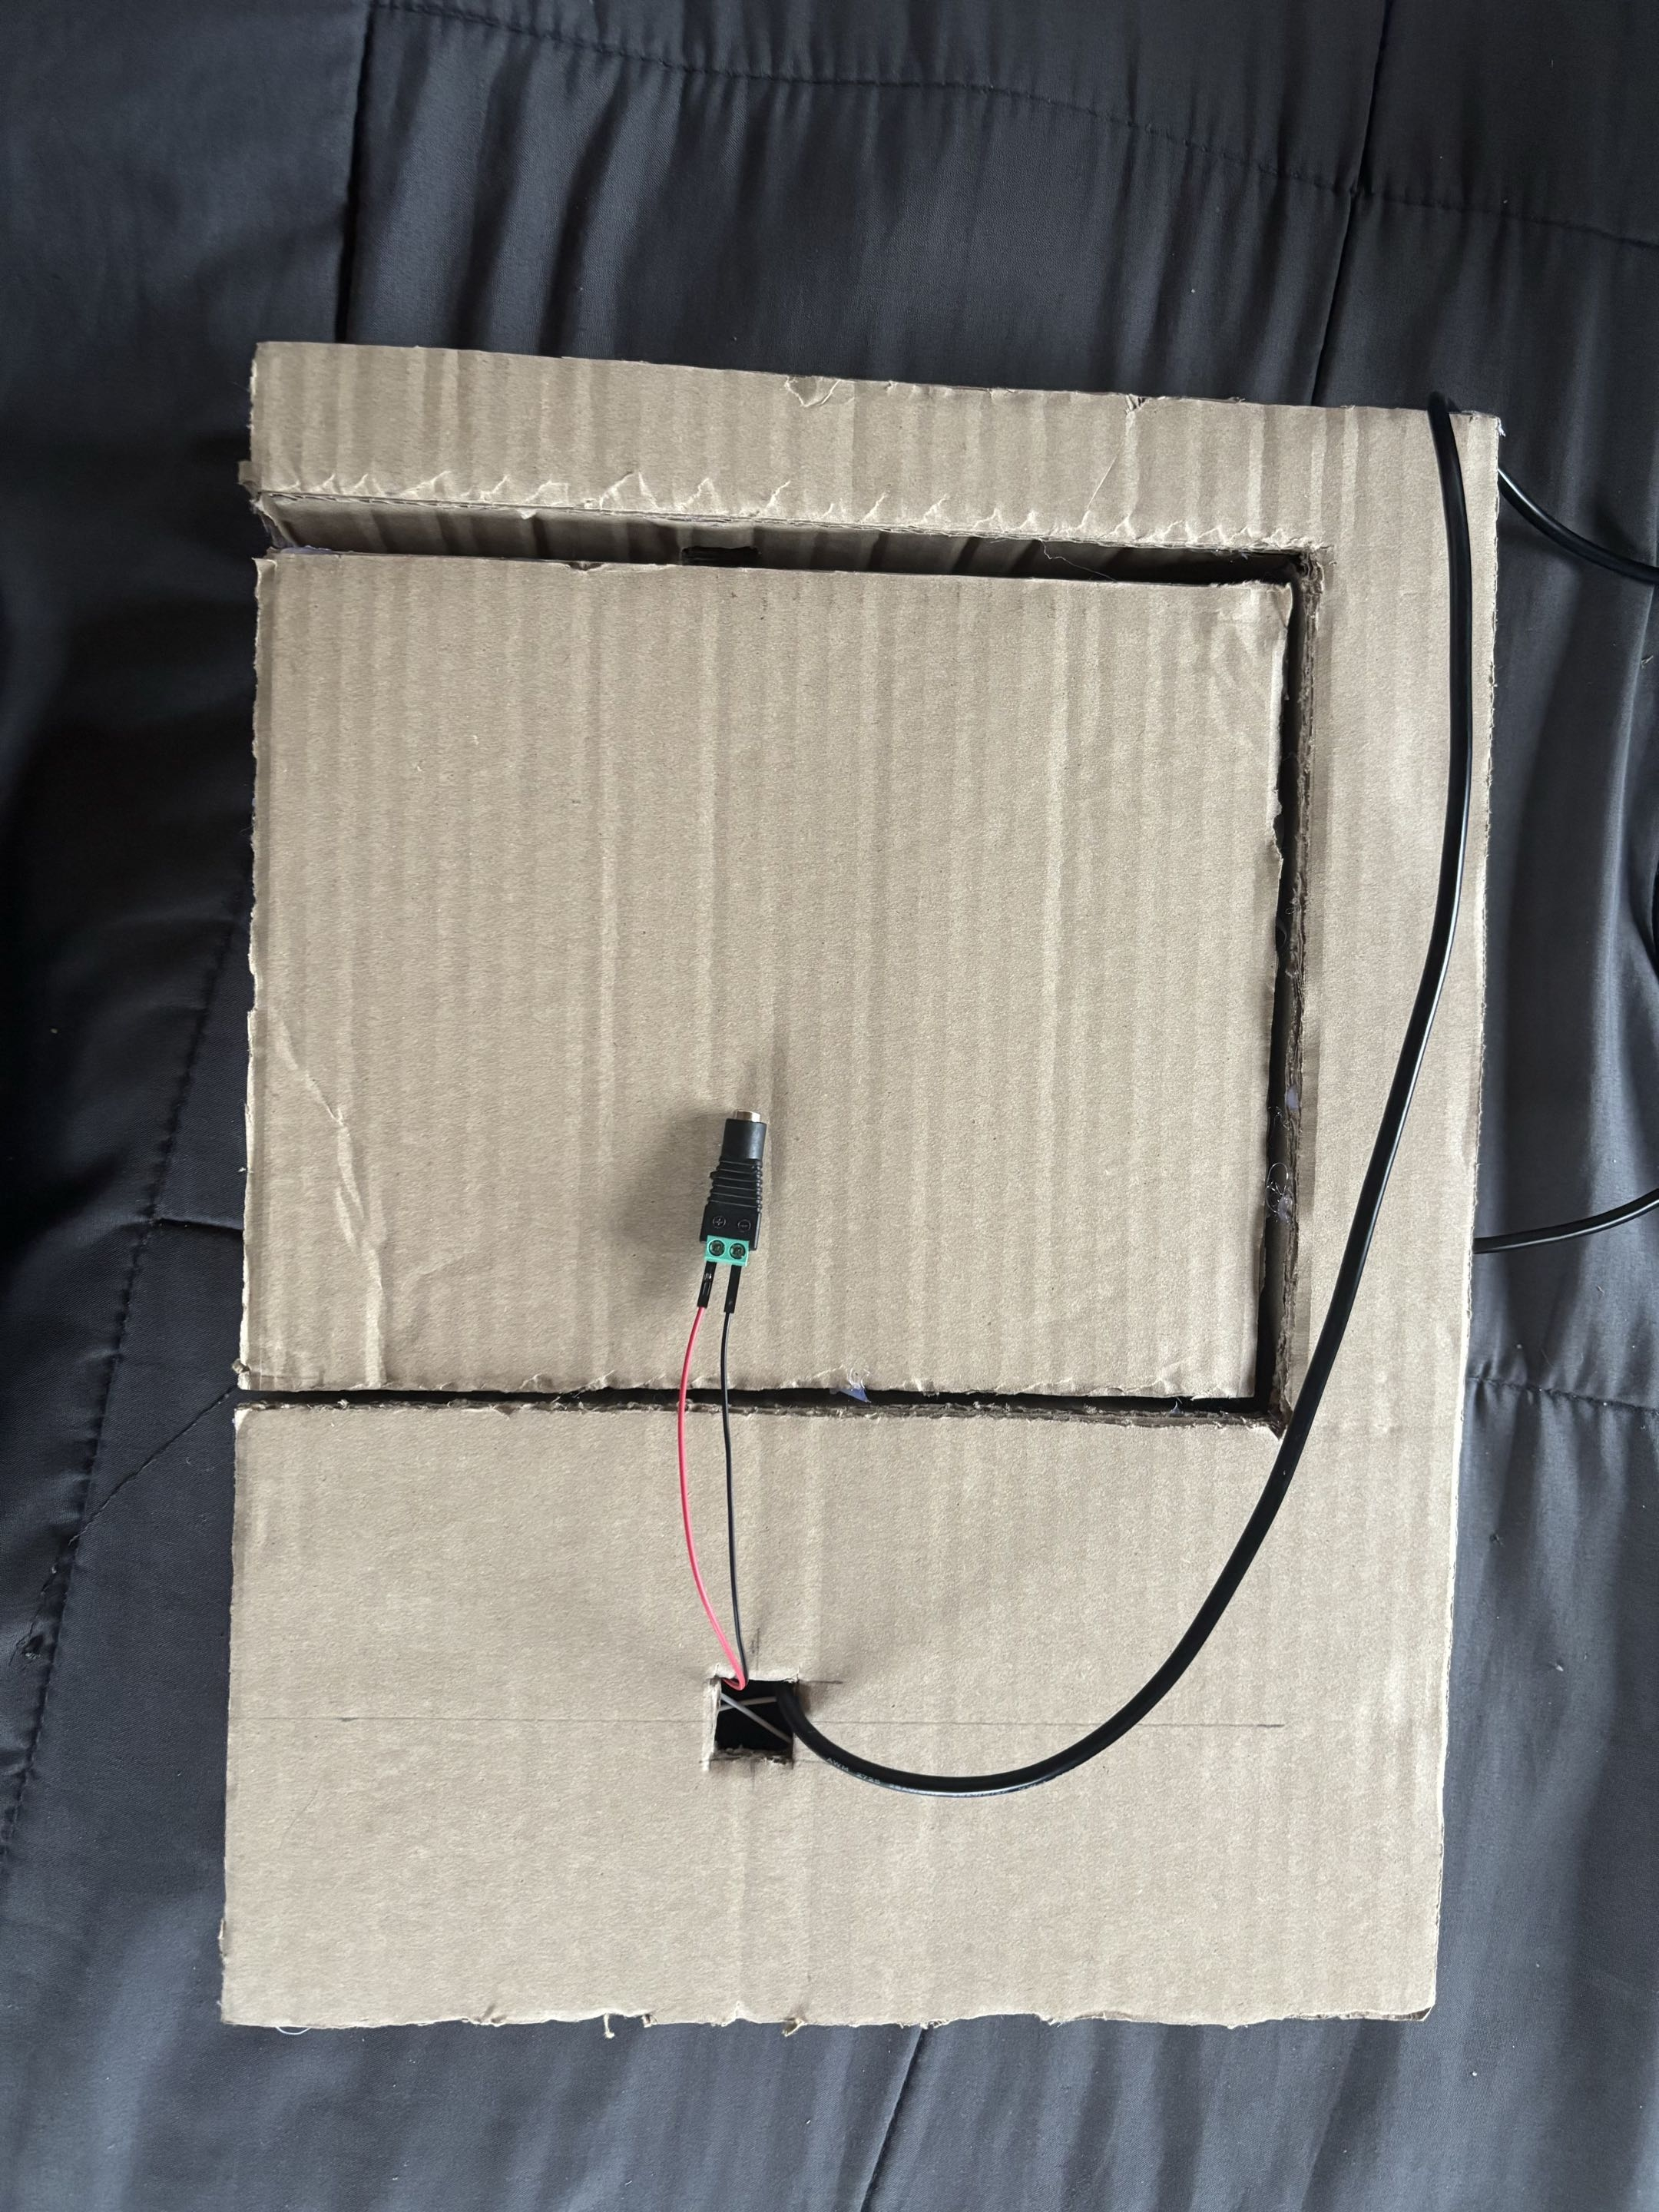
\includegraphics[width=0.6\linewidth]{Img/imagen1}
		\caption{vista trasera}
	\end{subfigure}
	\hfill
	\begin{subfigure}{0.45\textwidth}
		\centering
		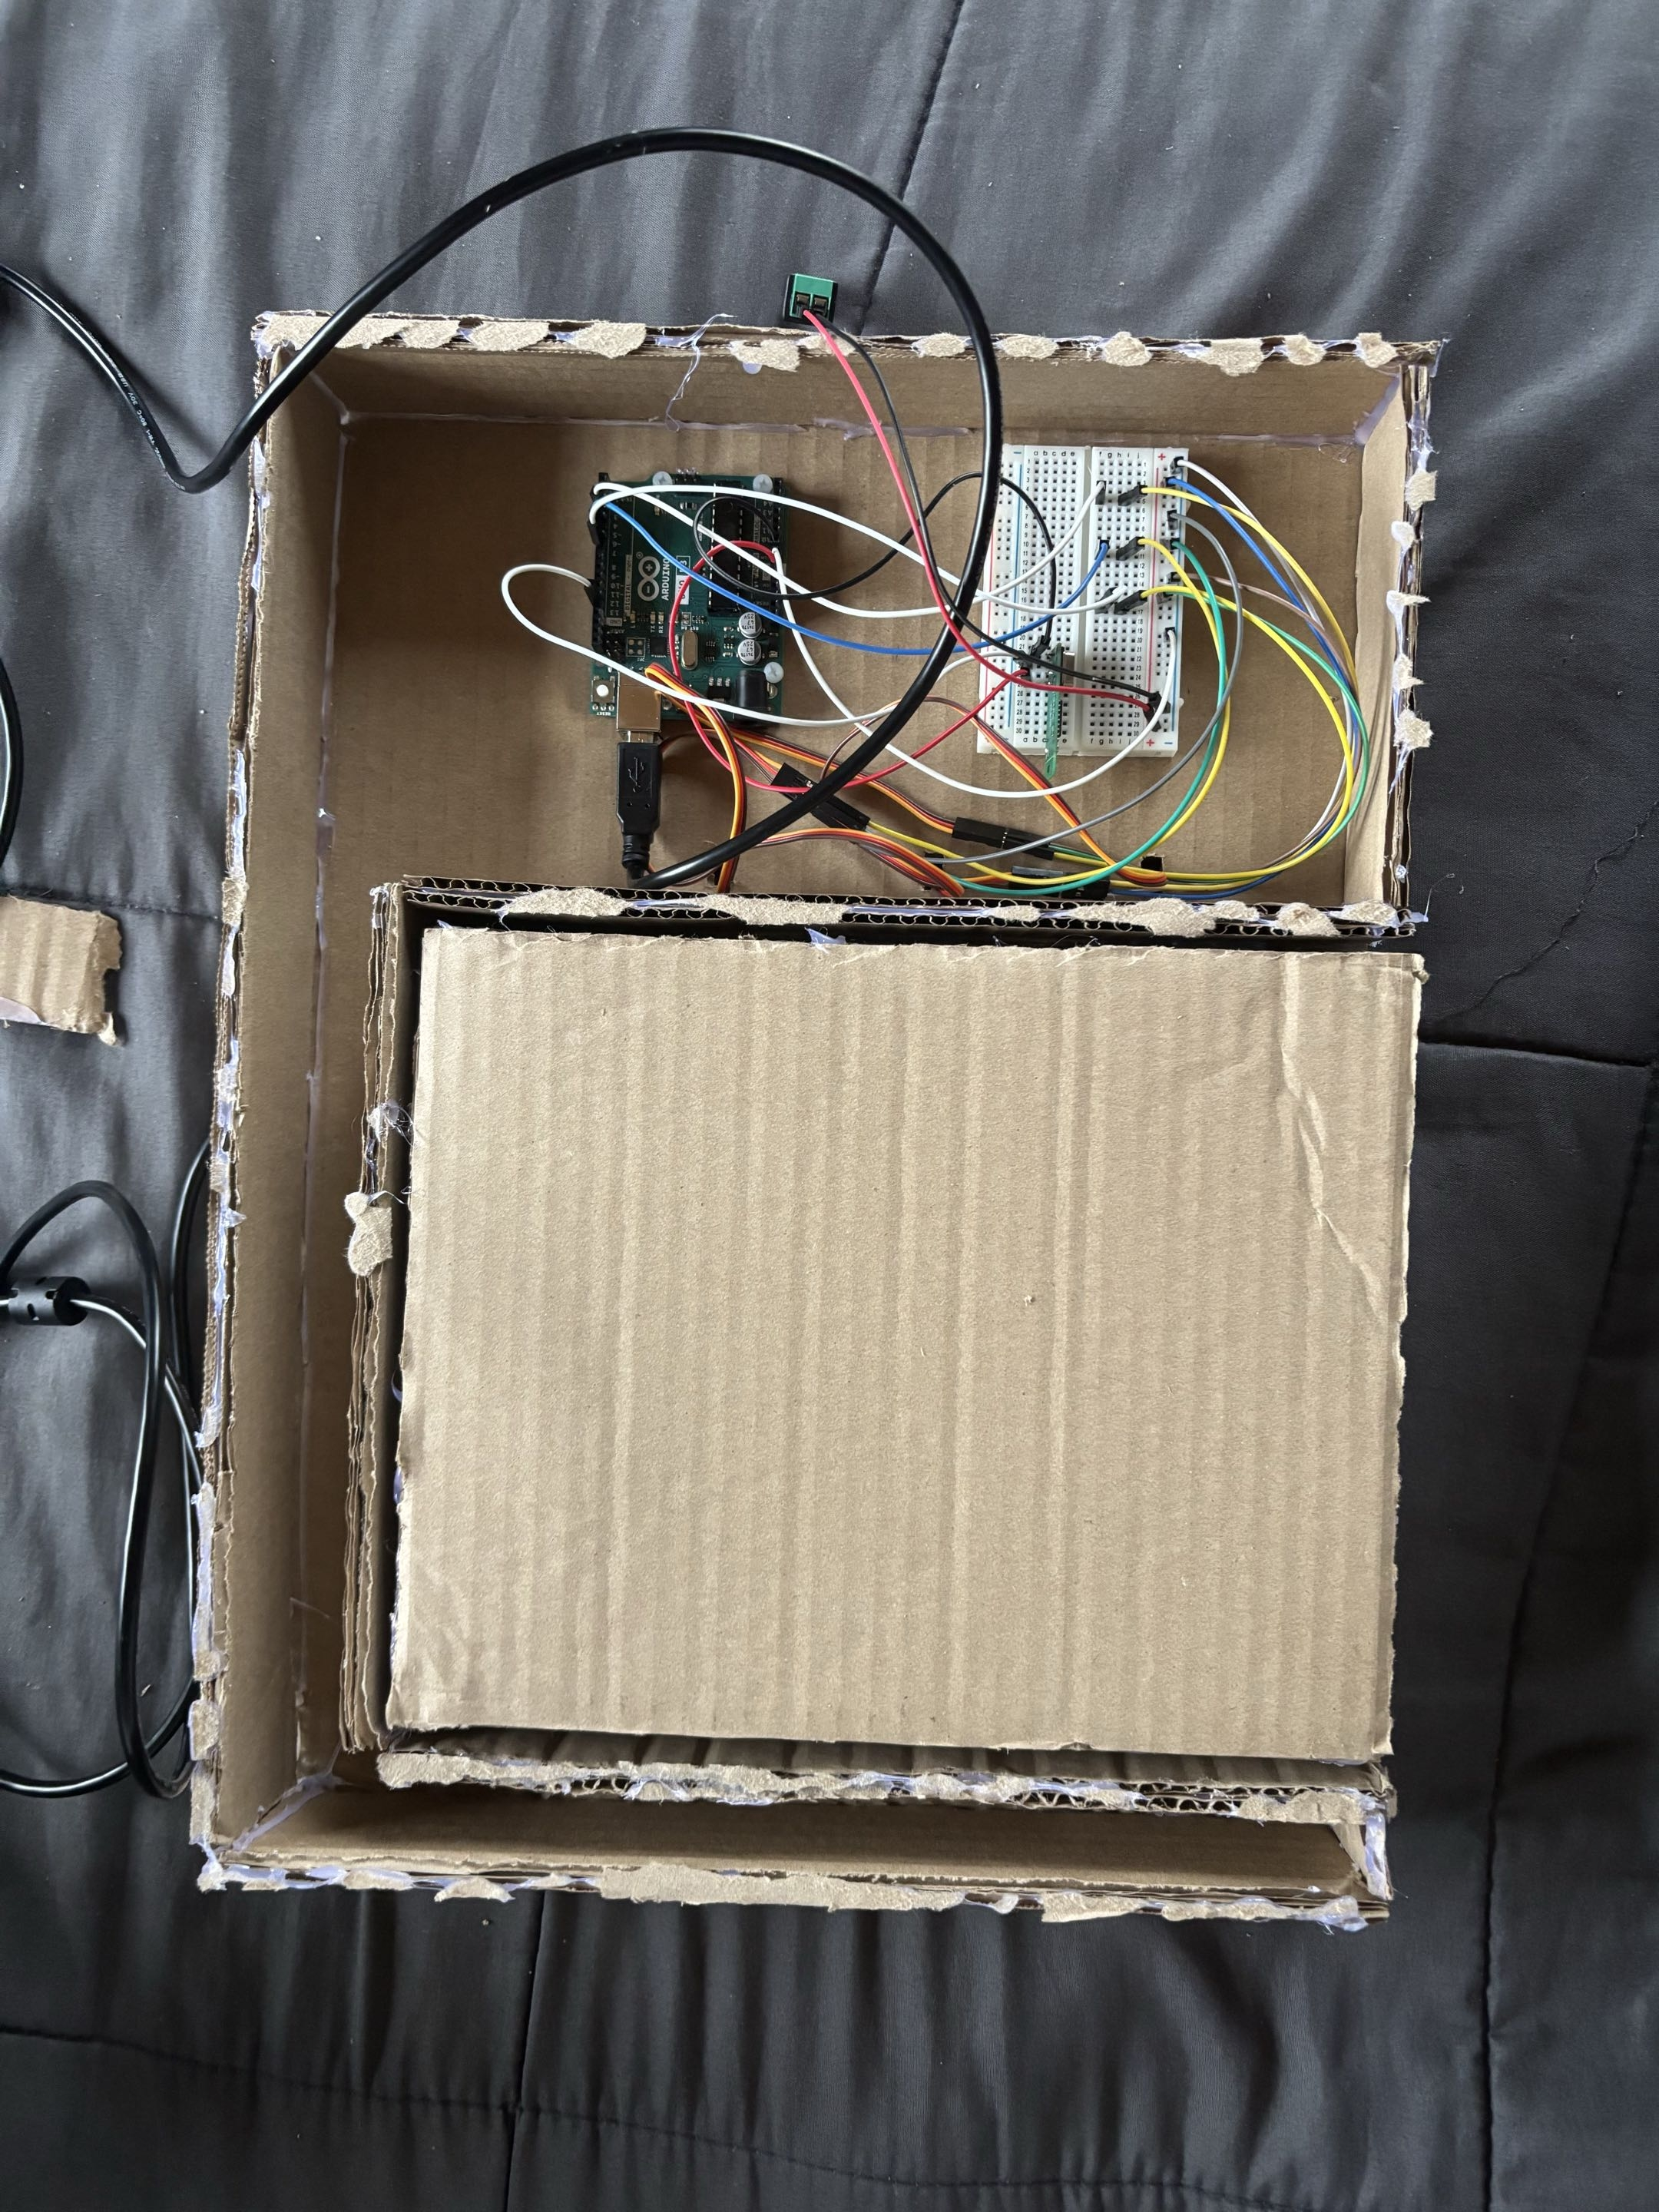
\includegraphics[width=0.6\linewidth]{Img/imagen7}
		\caption{vista interior parte servos}
	\end{subfigure}
	\hfill
	\begin{subfigure}{0.45\textwidth}
		\centering
		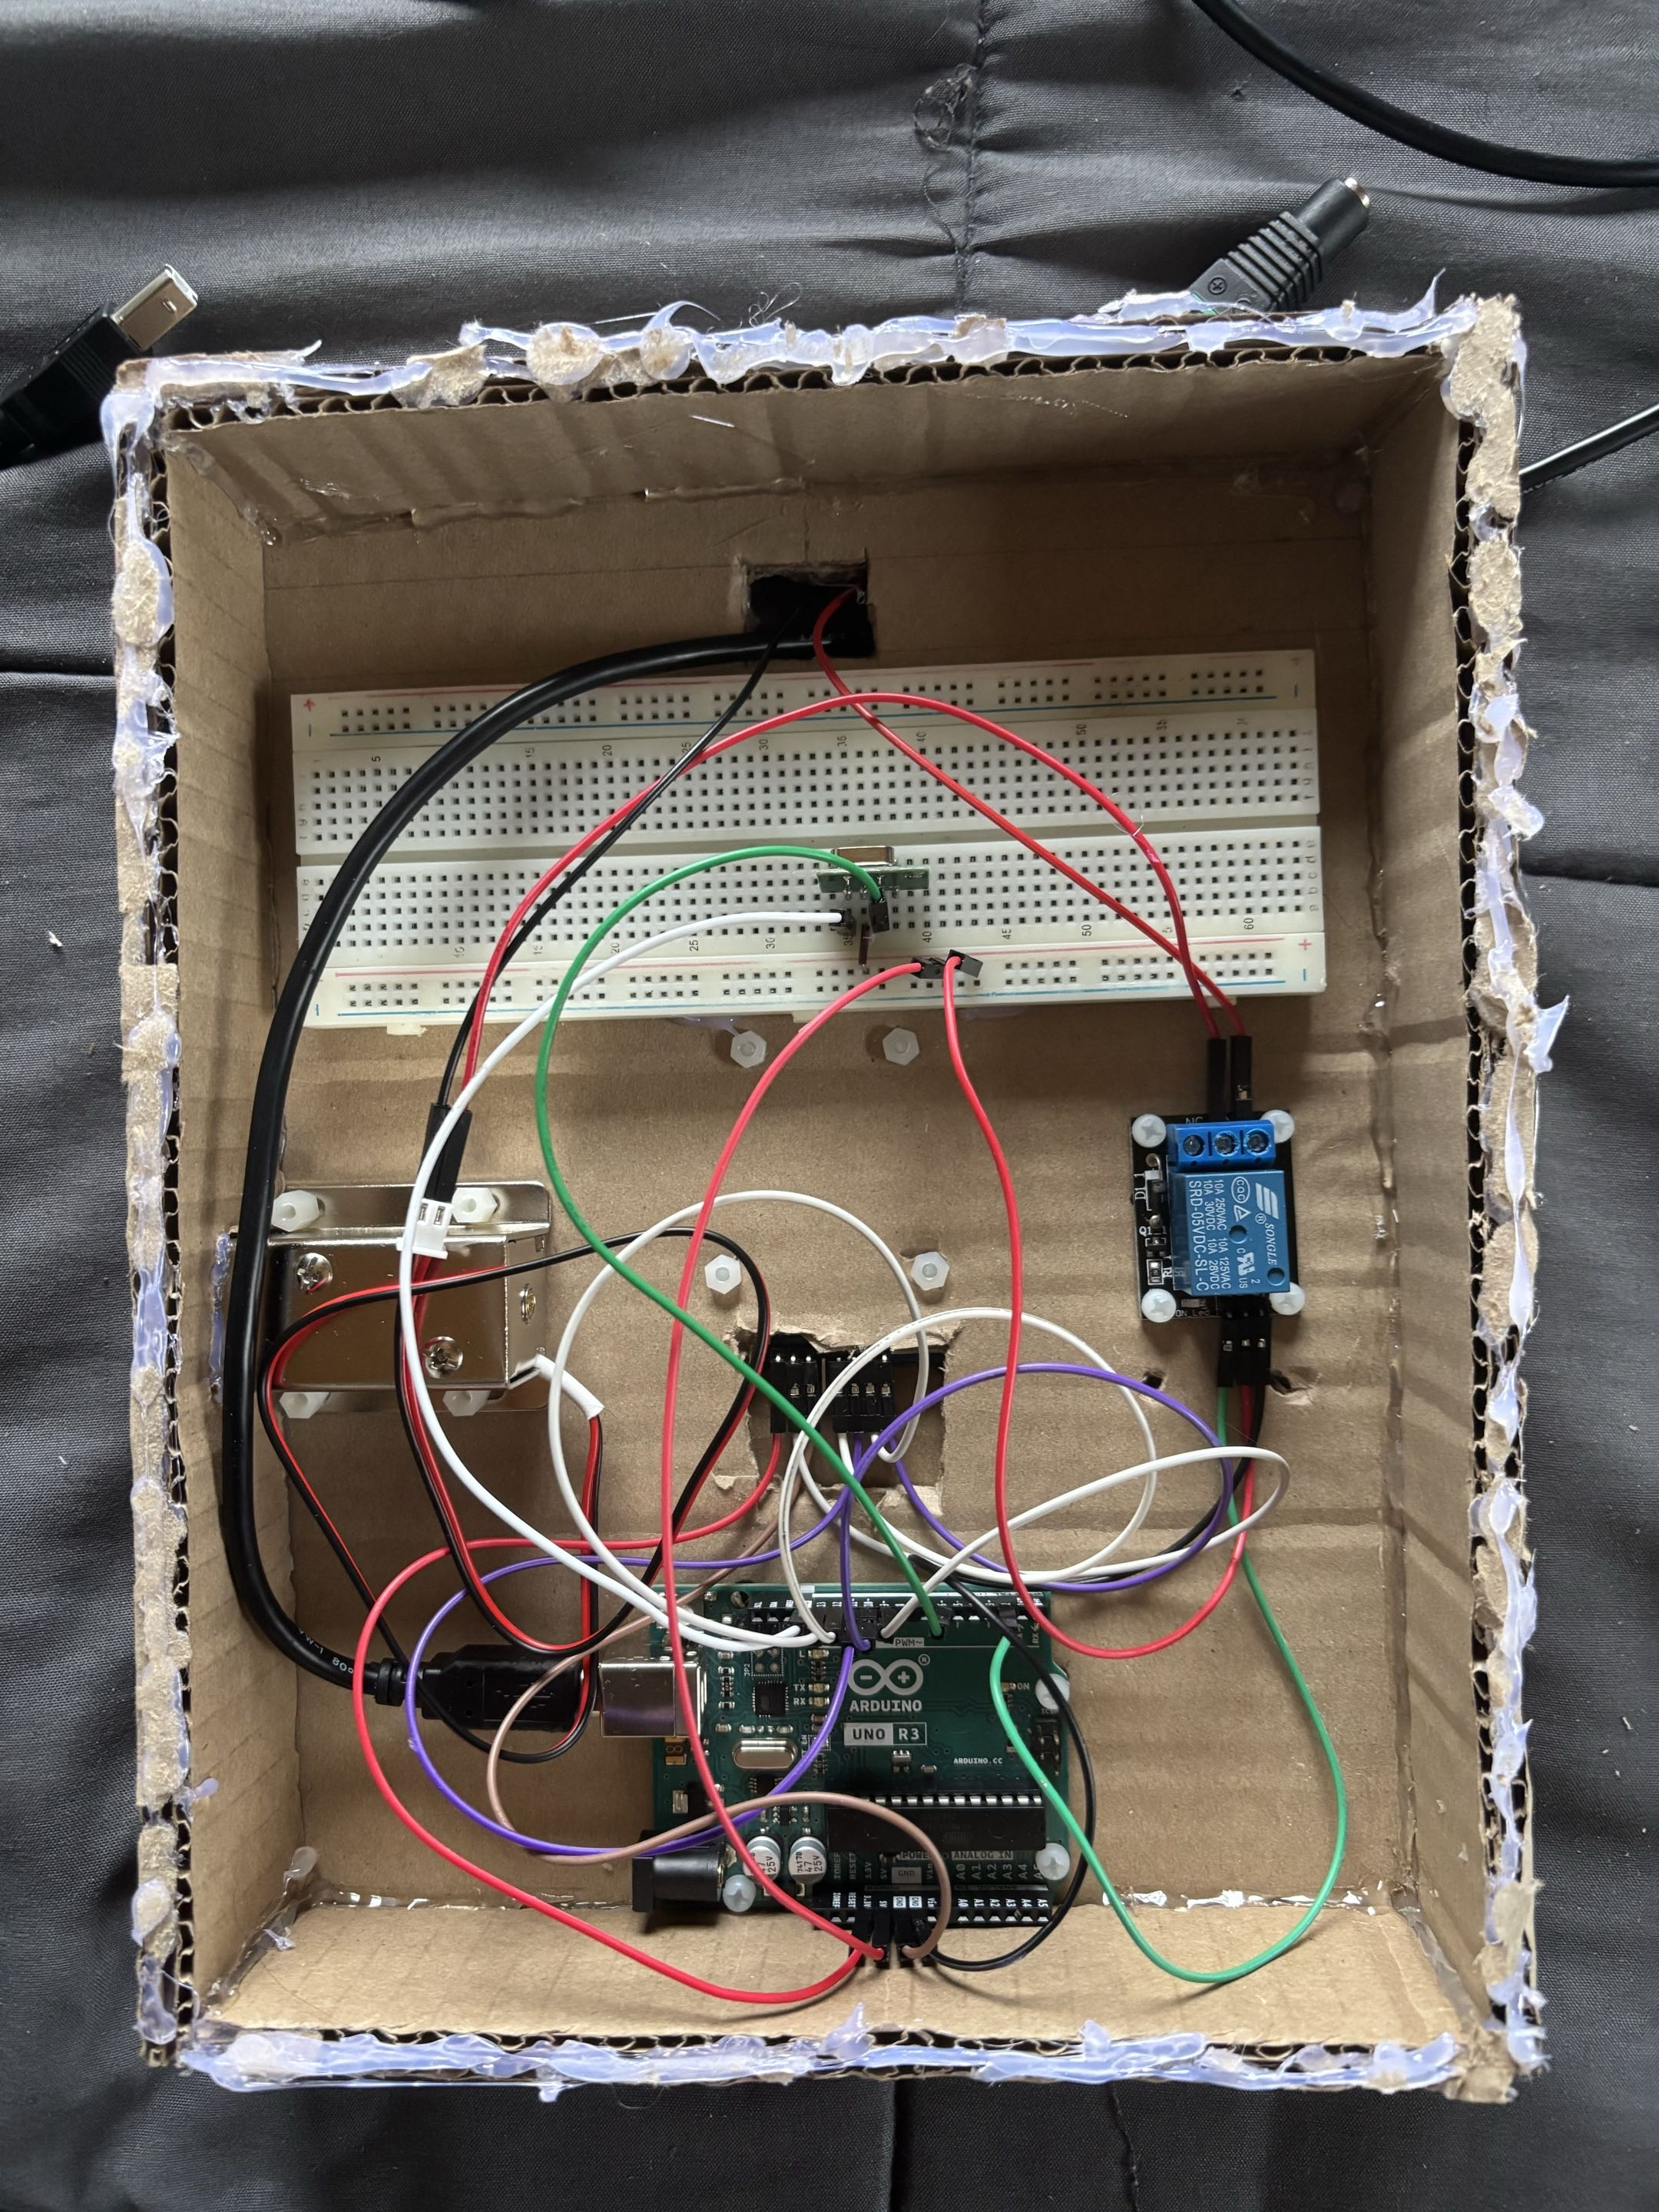
\includegraphics[width=0.6\linewidth]{Img/imagen5}
		\caption{vista interior puerta}
	\end{subfigure}
	\hfill
	\begin{subfigure}{0.45\textwidth}
		\centering
		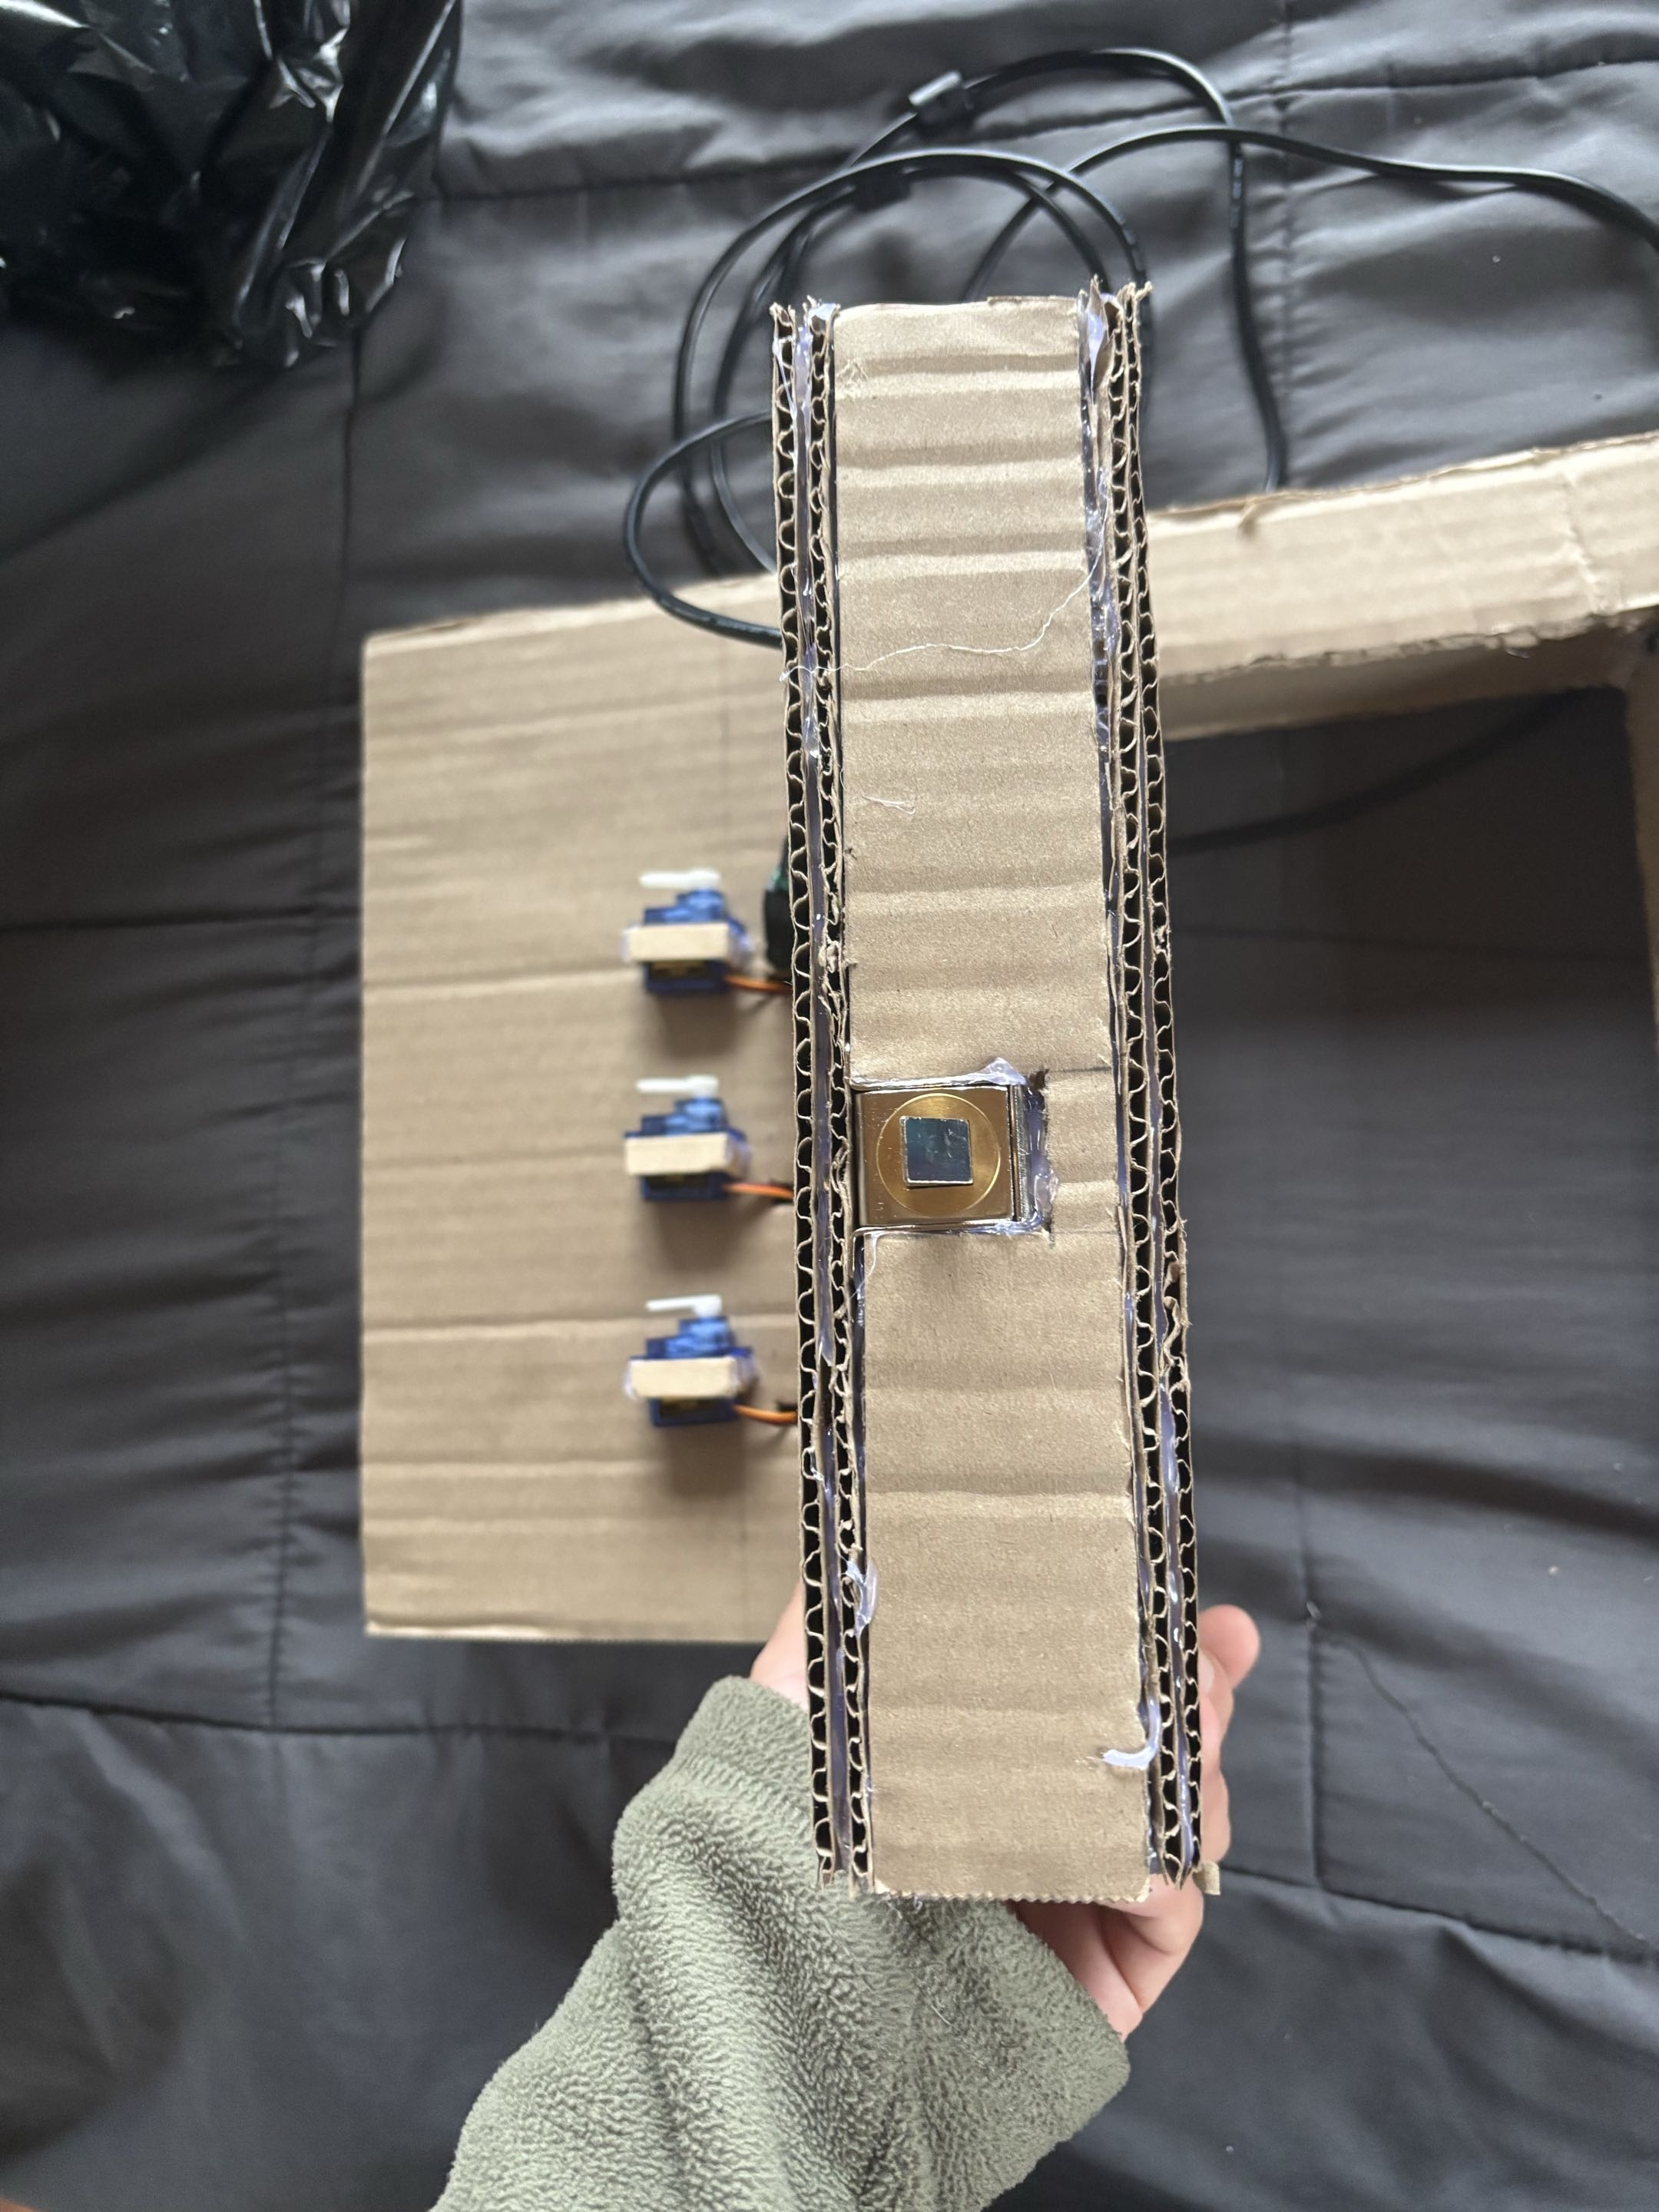
\includegraphics[width=0.6\linewidth]{Img/imagen4}
		\caption{vista pestillo}
	\end{subfigure}
	\hfill
	\begin{subfigure}{0.45\textwidth}
		\centering
		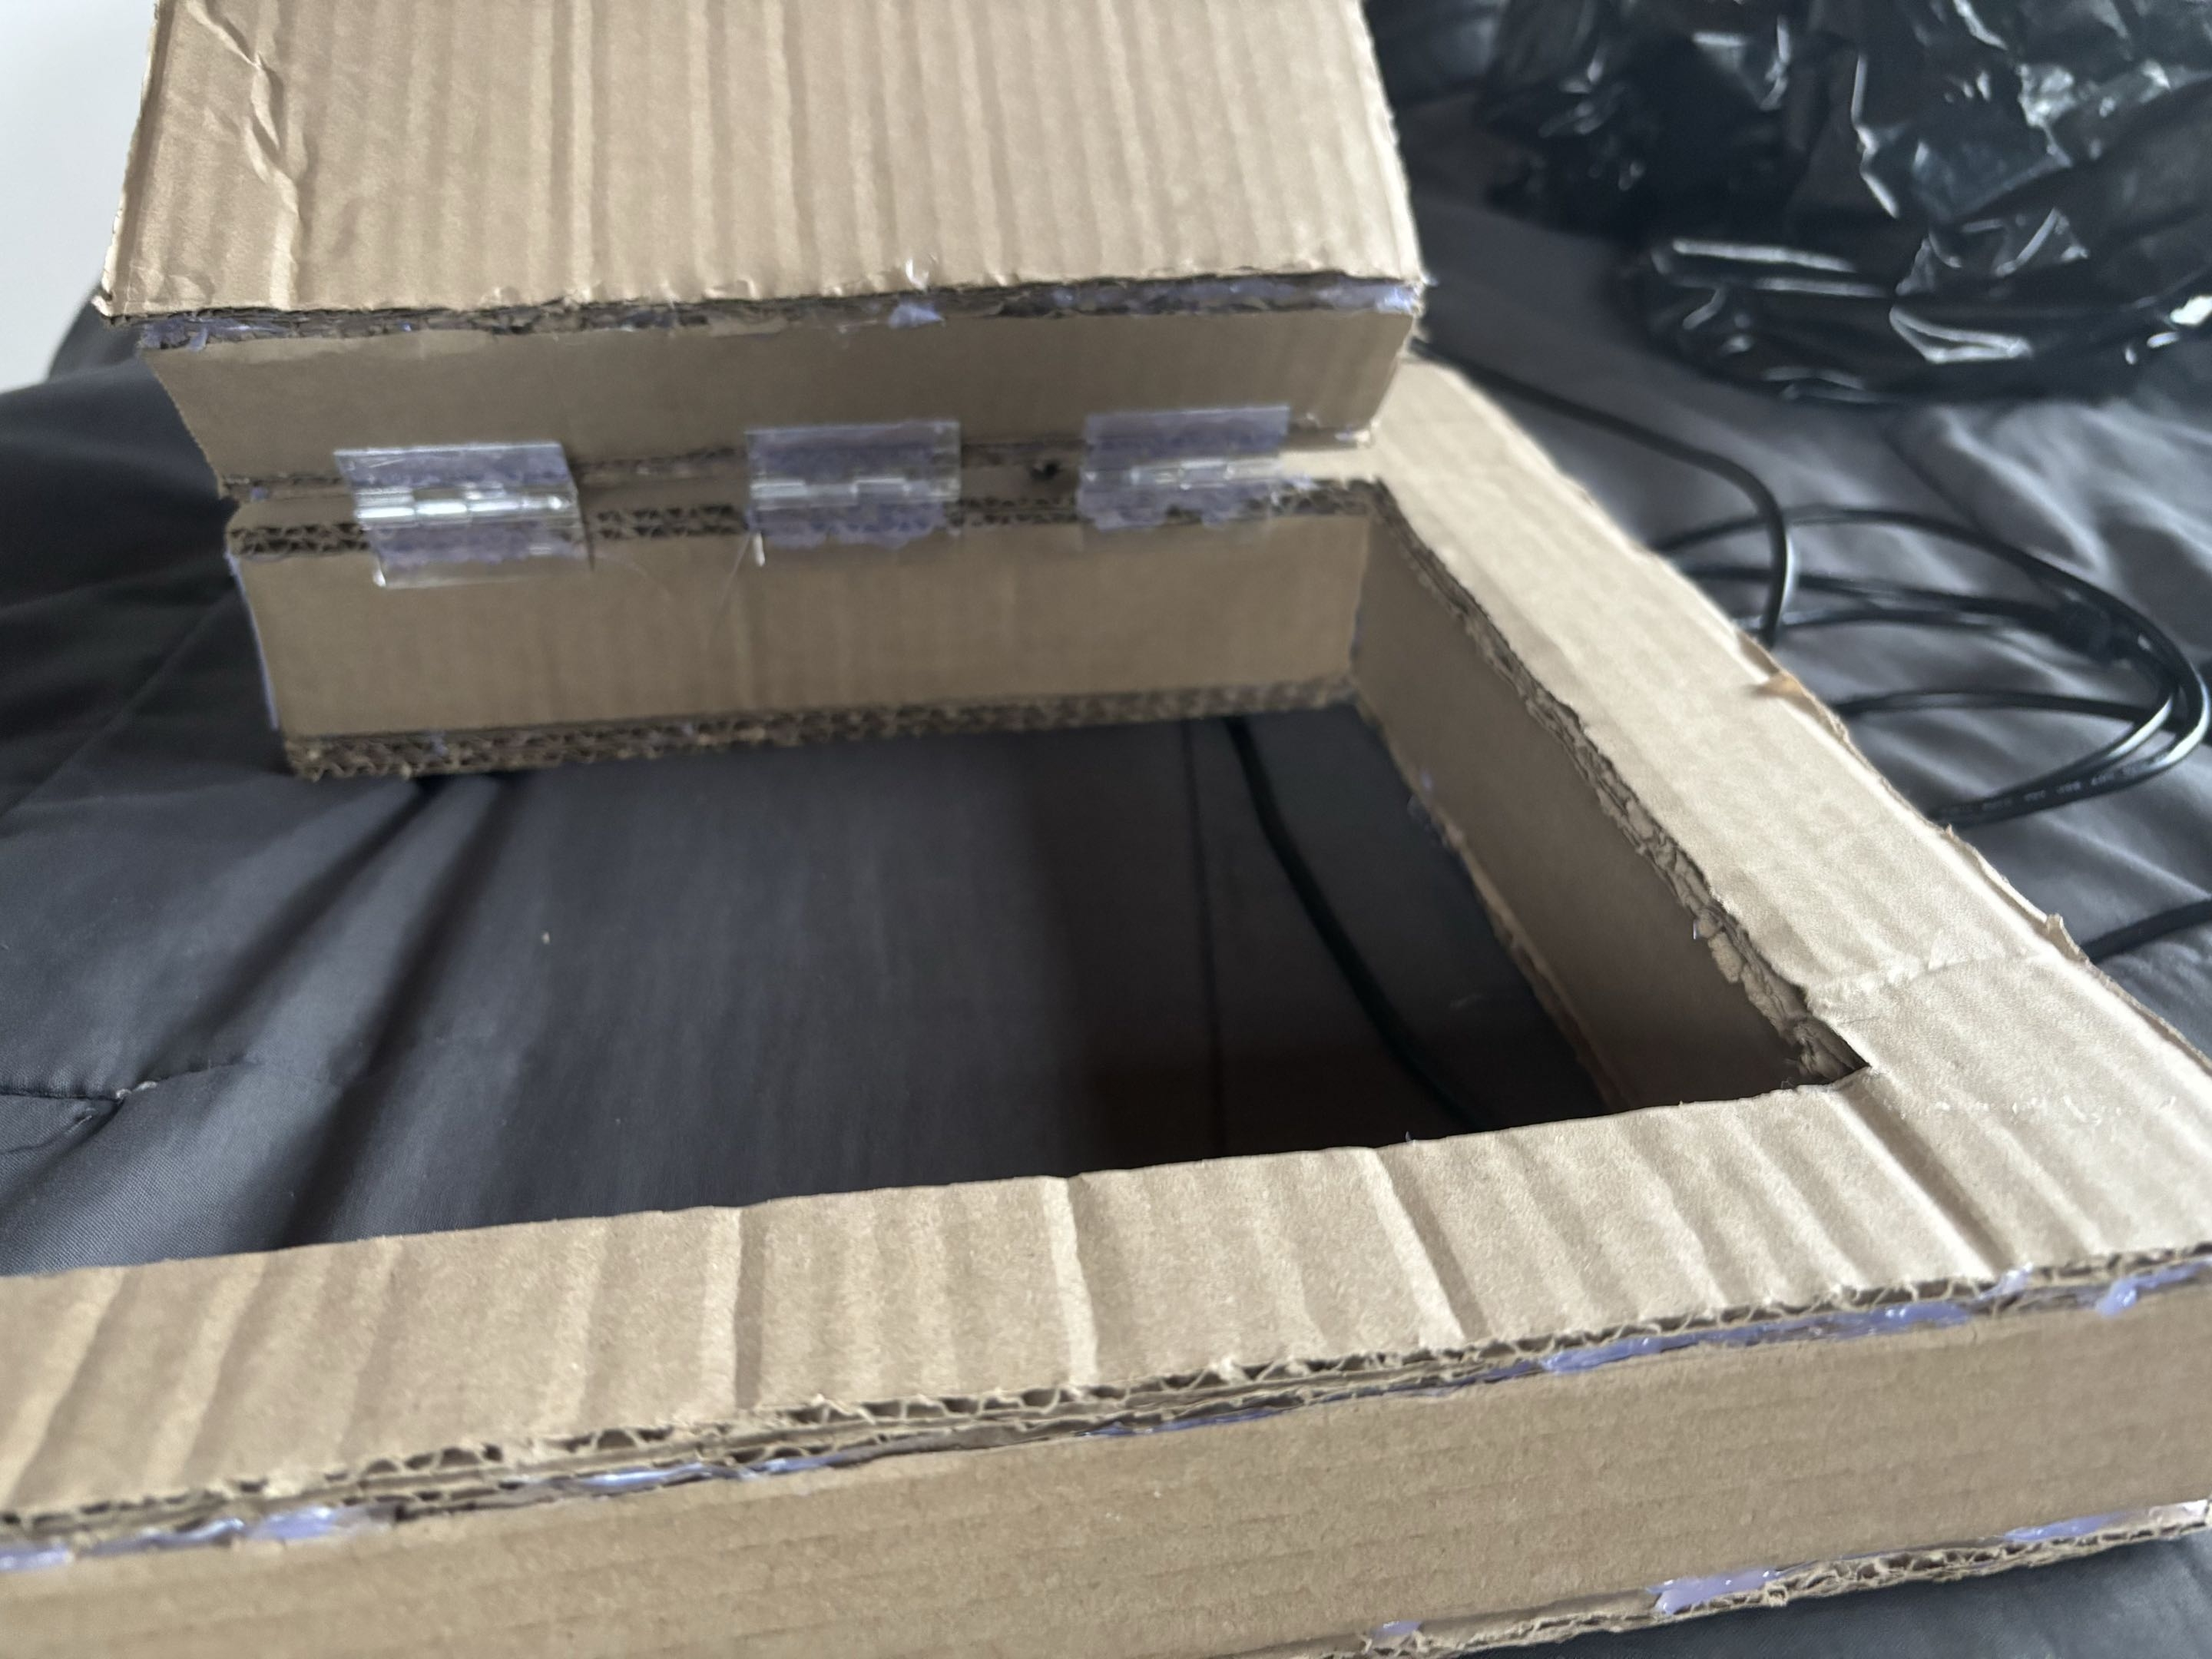
\includegraphics[width=0.6\linewidth]{Img/imagen3}
		\caption{vista bisagras}
	\end{subfigure}
\end{figure}
\end{document}